% Provenance (never printed): see sources/outline_sources.md (Year 1: elastic rebound and the
% seismic cycle; seismic moment and magnitudes; focal mechanisms; geodetic measurement of
% active deformation; the Gutenberg--Richter law). Exercise and problem values in the Book 3
% scratch calculator calc/ch18.py; figure data from figdata/bachelor-1/gutenberg_richter.py,
% beachballs.py and interseismic.py. Focus, epicentre, magnitude, intensity and seismometer
% are owned by Book 1 g7 (magnitude re-founded here as the moment magnitude); P and S waves by
% Book 2 g11; fault types and rake by ch. 17; stress, Coulomb and the seismogenic layer by
% ch. 16; the shear modulus by physics. Radar interferometry and the stereographic projection
% belong to later volumes (told, not defined).
\chapter{مصدر الزلزال}\label{ch:b1:earthquake-source}

% ledger: pp1515:1906, reid:1910
في صباح 18 أبريل 1906، انكسرت الأرض شمال سان فرانسيسكو وجنوبها على امتداد يزيد على أربعمائة كيلومتر. وقُطعت الطرق والأسوار وصفوف الأشجار التي عبرت الخطّ، ووُجد نصفا كلٍّ منها على بُعد أمتار، والنصف الغربي مزاح دائمًا نحو الشمال. وكان المساحون قد قاسوا مواضع المعالم في المنطقة طوال نصف القرن السابق، فلما قيست المعالم من جديد، أظهرت المقارنة شيئًا أغرب من الانكسار نفسه: فقد كانت الأرض تنحني، ببطء وسلاسة، لعقود قبل الزلزال، وكان الزلزال قد أتاح لها أن ترتدّ. يتتبّع هذا الفصل زلزالًا من التحميل البطيء لصدع إلى الدقائق القليلة التي ينزلق فيها، ويقرأ الانزلاق من الموجات ومن الأرض: كم كان كبيرًا، وفي أيّ اتجاه تحرّك، وكم بسرعة يُعدّ الزلزال التالي، وكم مرّة تأتي زلازل كلّ حجم.

\begin{recall}
بؤرة الزلزال هي النقطة التي يبدأ عندها الانكسار، ومركزه السطحي النقطة التي فوقها على السطح؛ والقدر يقيس حجم الزلزال، والشدّة تقيس الاهتزاز في مكان ما؛ ويسجّل مقياس الزلازل حركة الأرض كمخطّط زلزالي (الكتاب الأول، الصف السابع).
تصل موجة P، وهي موجة ضغط، أولًا، وتصل موجة S، وهي موجة قصّ، بعدها (الكتاب الثاني، الصف الحادي عشر). وللصدع جدار علوي \omterm{def:b1:faults-folds-fabrics:fault-elements}{وجدار مرتكز}؛ \omterm{def:b1:faults-folds-fabrics:fault-elements}{ومتجهة الانزلاق} هي إزاحة الجدار العلوي بالنسبة \omterm{def:b1:faults-folds-fabrics:fault-elements}{للجدار المرتكز}، وزاوية انزلاقها $r$ تُقاس على مستوى الصدع من \omterm{def:b1:geological-maps:attitude}{الامتداد}، وتسمّي \omterm{def:b1:faults-folds-fabrics:fault-elements}{زاوية الانزلاق} الصدع: نحو \ang{90} معكوس، ونحو \ang{-90} عادي، ونحو 0 \omterm{def:b1:faults-folds-fabrics:fault-types}{أيسر}، ونحو \ang{180} \omterm{def:b1:faults-folds-fabrics:fault-types}{أيمن} (\cref{ch:b1:faults-folds-fabrics}).
الصخر المرن يعود إلى شكله حين تُزال الإجهادات؛ ومعامل القص $\mu$ يربط إجهاد القص \omterm{def:b1:stress-strain-rheology:strain}{بانفعال القصّ} الذي يُولّده (الفيزياء)؛ وتنزلق الصدوع حين يبلغ إجهاد القصّ متانتها الاحتكاكية، وتبدأ الزلازل في الجزء الهشّ العلوي من \omterm{def:b1:layered-earth:layers}{القشرة}، أي \omterm{def:b1:stress-strain-rheology:strength-envelope}{الطبقة المولّدة للزلازل} (\cref{ch:b1:stress-strain-rheology}). وتقيس محطات تحديد المواقع الدائمة بالأقمار الصناعية، التي تعطي مواضعها اليومية على مدى سنوات سرعةَ الأرض عند موقعها، حركاتِ الصفائح (\cref{ch:b1:plate-kinematics}).
\end{recall}

\section{الارتداد المرن والدورة الزلزالية}\label{sec:b1:earthquake-source:cycle}

صفيحتان تنزلقان إحداهما بجوار الأخرى بمعدّل ثابت، لا تنزلقان عادةً انزلاقًا ثابتًا على الصدع بينهما. فالاحتكاك يُبقي الصدع مقفلًا بينما تستمرّ الصفيحتان في الحركة بعيدًا عنه، فتنحني الصخور على جانبيه كنابض. فحين يبلغ إجهاد القصّ على الصدع متانته، ينزلق الصدع في ثوانٍ أو دقائق، فترتدّ الصخور المنحنية.

\begin{definition}[الارتداد المرن، والدورة الزلزالية، وفترة التكرار]\label{def:b1:earthquake-source:seismic-cycle}
\emph{الارتداد المرن}\index{ارتداد مرن} هو عودة الصخور على جانبي الصدع فجأةً نحو شكلها غير المجهد، حين ينزلق الصدع، الذي كان مقفلًا أثناء تجهيدها، في زلزال؛ فتُطلَق الطاقة المرنة المخزونة فيها، جزئيًّا في موجات زلزالية. و\emph{الدورة الزلزالية}\index{الدورة الزلزالية} لقطعة من الصدع هي التعاقب المتكرّر لمرحلة طويلة بين الزلازل، تبقى فيها القطعة مقفلةً فيتراكم حولها الانفعال، ومرحلة مشاركة للزلزال، ينزلق فيها الصدع، ومرحلة ما بعد الزلزال، من شهور إلى عقود، يتكيّف فيها المحيط مع الحالة الجديدة. و\emph{فترة التكرار}\index{فترة التكرار} لقطعة من الصدع هي الزمن بين زلزالين كبيرين متتابعين عليها.
\end{definition}
% ledger: usgs:gloss-rebound, reid:1910, usgs:pp1515-thatcher

\begin{omfigure}
\begin{tikzpicture}[>={Stealth[length=5pt]}, font=\small]
% map view of a fence across a locked dextral strike-slip fault (north up): (a) built straight;
% (b) after decades of loading, bent with the interseismic profile v(x) = -(s/pi) arctan(x/D)
% (dextral: the east side moves south); (c) after the earthquake, straight again on each side and
% offset by s at the fault. Panel 3.4 cm wide (x from -1.7 to 1.7 cm), D = 0.35 cm, s = 0.9 cm.
\def\s{0.9}\def\Dl{0.35}
\foreach \k/\t in {0/{(أ) السور مبنيّ}, 1/{(ب) عقود من التحميل}, 2/{(ج) بعد الزلزال}} {
  \begin{scope}[xshift=\k*4.6cm]
    \fill[omLithSand!25] (-1.7,-1.6) rectangle (1.7,1.6);
    \draw[black!50, line width=0.4pt] (-1.7,-1.6) rectangle (1.7,1.6);
    \draw[fault, line width=1.1pt] (0,-1.6) -- (0,1.6);
    \node[anchor=north, align=center, font=\scriptsize] at (0,-1.7) {\t};
    % far-field motion of the two blocks, relative to the fault
    \draw[->, omThm, line width=0.8pt] (-1.35,-1.25) -- (-1.35,-0.45);
    \draw[->, omThm, line width=0.8pt] (1.35,1.25) -- (1.35,0.45);
    \ifnum\k=0
      \draw[line width=1.2pt, omDef] (-1.7,0) -- (1.7,0);
    \fi
    \ifnum\k=1
      \draw[line width=1.2pt, omDef] plot[domain=-1.7:1.7, samples=81, variable=\x] (\x, {-\s/pi*atan(\x/\Dl)*pi/180});
      \draw[black!45, dashed, line width=0.4pt] (-1.7,0) -- (1.7,0);
    \fi
    \ifnum\k=2
      \draw[line width=1.2pt, omDef] (-1.7,{\s/2}) -- (0,{\s/2});
      \draw[line width=1.2pt, omDef] (0,{-\s/2}) -- (1.7,{-\s/2});
      \draw[black!45, dashed, line width=0.4pt] (-1.7,0) -- (1.7,0);
      \draw[<->, line width=0.5pt] (0.18,{\s/2}) -- (0.18,{-\s/2});
      \node[anchor=west, font=\scriptsize] at (0.2,0.12) {الانزلاق};
    \fi
  \end{scope}
}
\node[anchor=south, font=\scriptsize] at (0,1.62) {الصدع};
\draw[->, line width=0.5pt] (-1.5,0.75) -- (-1.5,1.15) node[above, font=\scriptsize, inner sep=1pt] {ش};
\end{tikzpicture}
\par\smallskip{\small \omterm{def:b1:earthquake-source:seismic-cycle}{الارتداد المرن} مرئيًّا من الأعلى، على سور (أزرق) مبنيّ مستقيمًا عبر صدع \omterm{def:b1:faults-folds-fabrics:fault-types}{أيمن} مقفل. الأسهم الحمراء: حركة الكتلتين بعيدًا عن الصدع، بالنسبة له. (ب) والصدع مقفل: تتحرّك الأرض البعيدة ويُنحني السور، على امتداد منحنى الانحناء البيني ل\cref{sec:b1:earthquake-source:geodesy}. (ج) يُطلِق الزلزال الانحناء: كل نصف من السور مستقيم من جديد، ويتزحزح النصفان عند الصدع بقدر الانزلاق. والانحناء مبالغ فيه: فالسور الحقيقي ينحني بضعة أمتار على عشرات الكيلومترات.}
\label{fig:b1:earthquake-source:rebound}
\end{omfigure}

إن كان الصدع مقفلًا بين الزلازل، وكان كل زلزال يلغي الانزلاق الذي تراكم منذ الزلزال الأخير، فإن حركة الصفائح تحدّد وتيرة الدورة.

\begin{proposition}[التكرار من معدّل الانزلاق]\label{prop:b1:earthquake-source:recurrence}
ليكن لقطعة من صدع معدّل انزلاق طويل المدى $\dot s$، وليكن مقفلًا بين الزلازل، وينزلق بالمقدار نفسه $D$ في كل زلزال. فإن \omterm{def:b1:earthquake-source:seismic-cycle}{فترة التكرار} لزلازلها هي
\[
  T = \frac{D}{\dot s} .
\]
وإن كان الكسر $c$ فقط من معدّل الانزلاق مقفلًا، والباقي ينزلق انزلاقًا ثابتًا دون زلازل، فإن $T = D/(c\,\dot s)$.
\end{proposition}

\begin{proof}
على مدى زمن طويل $t$، يتحرّك جانبا الصدع بالمقدار $\dot s\,t$ بالنسبة لبعضهما. وبعيدًا عن الصدع تتحرّك الأرض بانتظام، فعلى الصدع نفسه يجب أن تُعوَّض الإزاحة نفسها، وهنا بالزلازل وحدها: فإن وقع $N$ زلزال في الزمن $t$، فإن $N D = \dot s\,t$ حتى انزلاق زلزال واحد، و$t/N \to D/\dot s$. وإذ يحدث الكسر $1-c$ من الانزلاق بانزلاق ثابت، فإن الزلازل تعوّض $c\,\dot s\,t$، وتكون $t/N \to D/(c\,\dot s)$.
\end{proof}

مع قيم نموذجية لصدع سان أندرياس، انزلاق قدره \qty{4}{m} في كل زلزال كبير، ومعدّل انزلاق قدره \qty{20}{mm.yr^{-1}}، تكون \omterm{def:b1:earthquake-source:seismic-cycle}{فترة التكرار} \qty{200}{yr}. وعند جدول وولاس، في وسط كاليفورنيا، أُزيح مجرى جدول قطع الصدع بمقدار \qty{128}{m} خلال \num{3587} سنة منذ أن حُفر المجرى، أي بمتوسط \qty{36}{mm.yr^{-1}}، قريبًا من المعدّل نحو \qty{34}{mm.yr^{-1}} المقاس على إزاحات أخرى هناك؛ وآخر زلزال كبير على ذلك المقطع، عام 1857، انزلق بما يقارب \qty{10}{m}، وهذا يستغرق بهذا المعدّل نحو ثلاثة قرون لكي يتراكم.
% ledger: usgs:pp1515-thatcher, usgs:pp1515-wallace, commons:wallace-creek

\begin{omfigure}
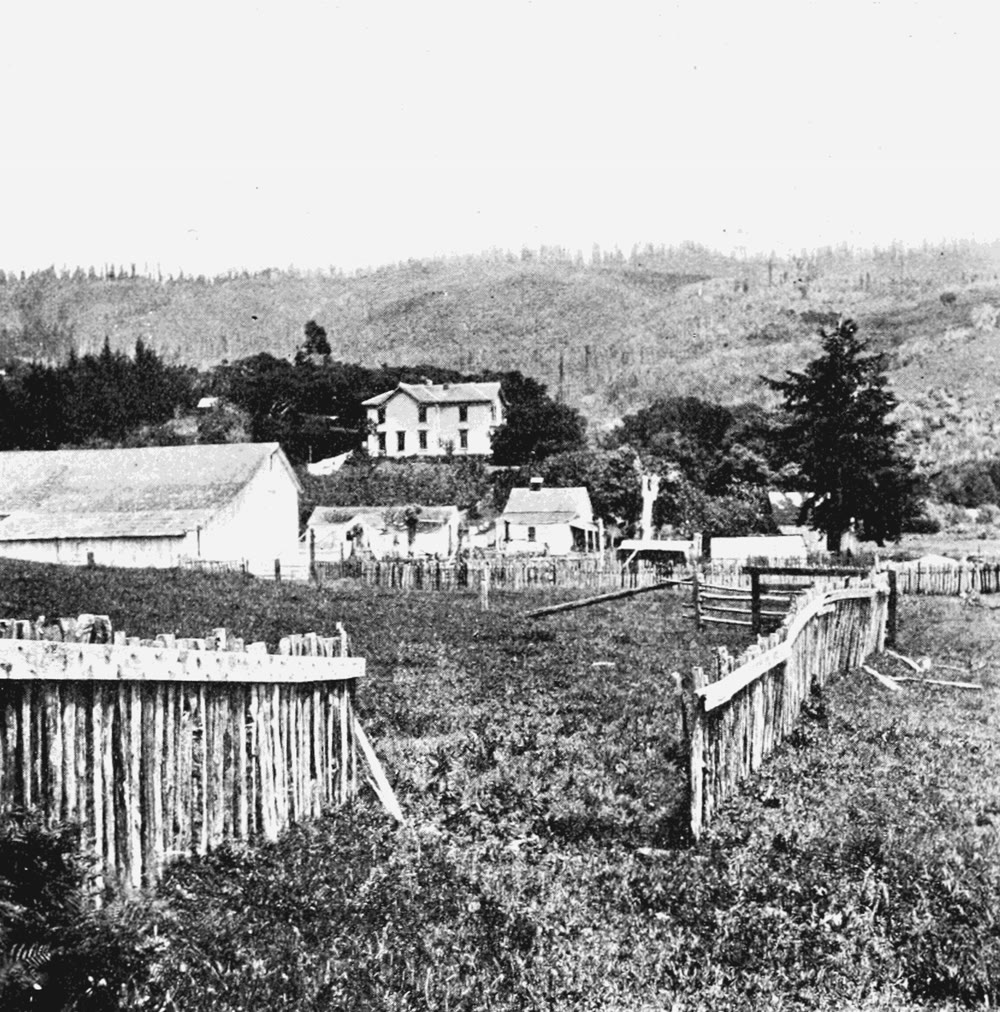
\includegraphics[height=5.6cm]{images/book3/b1-fence-1906.jpg}\hfill
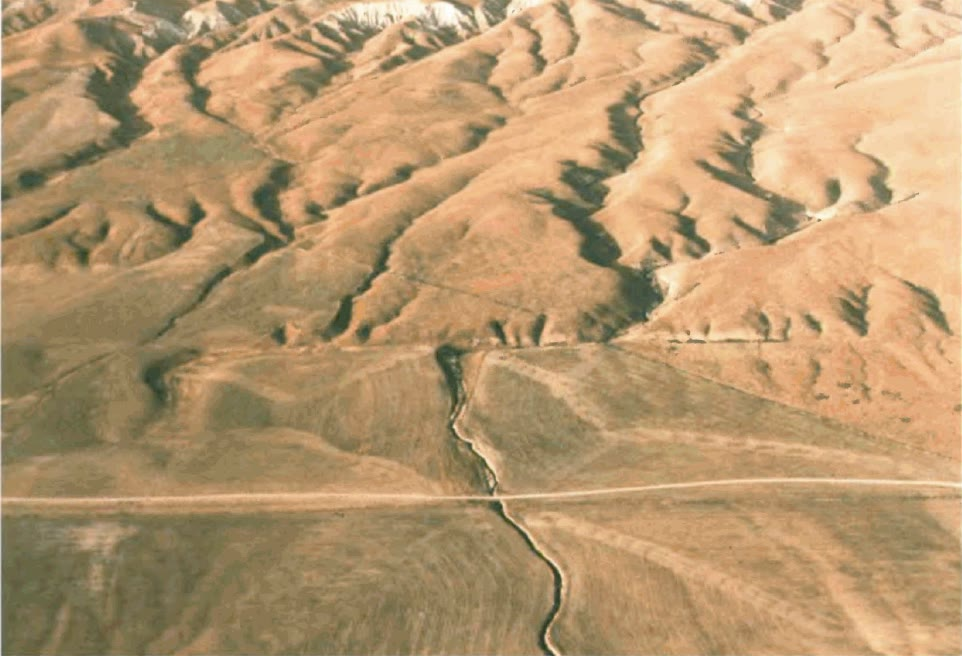
\includegraphics[height=5.6cm]{images/book3/b1-wallace-creek.jpg}
\par\smallskip{\small يسارًا: أسوار في أراضٍ زراعية في مقاطعة مارين، شمال سان فرانسيسكو، عبرها انكسار 1906، نُشرت في السنة نفسها بعنوان ``land separated by the earthquake fault''. تصوير من \emph{Popular Science Monthly}، vol.~69 (1906), ملك عام. ويمينًا: جدول وولاس، في كاريزو بلين، مرئيًّا من الجوّ: ينحدر الجدول من التلال (في الأعلى)، وحيث يعبر صدع سان أندرياس، عند سفح التلال، ينزاح مجراه جانبًا بمقدار \qty{130}{m}، وهي الإزاحة المتراكمة عبر آلاف السنين من الزلازل. تصوير: R.~E.~Wallace, U.S. Geological Survey, ملك عام. وكلتاهما من ويكيميديا كومنز.}
\label{fig:b1:earthquake-source:offsets}
\end{omfigure}
% ledger: commons:psm-fence, commons:wallace-creek

المقترح يعطي متوسّطًا، لا جدولًا زمنيًّا. فقرب باركفيلد، على الصدع نفسه، تبع زلزالًا بقدر نحو 6 عام 1857 خمسةُ زلازل أخرى تشبهه، على المقطع نفسه، على مسافة نحو \qty{30}{km}، بفواصل نحو 22 سنة حتى عام 1966؛ وكان من المتوقَّع الزلزال التالي قبل 1993، لكنه وقع عام 2004، بقدر عزم 6.0 ومن دون أي علامة إنذار واضحة. فمتانة الصدع، وانزلاق كل زلزال، وتحميله من جيرانه، كلها تتغيّر من دورة إلى أخرى، \omterm{def:b1:earthquake-source:seismic-cycle}{والدورة الزلزالية} توصف أفضل بمتوسّط \omterm{def:b1:earthquake-source:seismic-cycle}{فترة التكرار} وانتشار حوله، من وصفها بدور ثابت.
% ledger: pp1515:parkfield, bl85:parkfield, usgs:hist-mw, bakun:2005

بعض قطع الصدوع لا تُقفل البتّة. فبين باركفيلد وسان خوان بوتيستا يزحف القسم الأوسط من صدع سان أندرياس: فالانزلاق الثابت على الصدع يستوعب تقريبًا كل حركة الصفيحتين، ولا يتراكم إلا القليل من الانفعال على جانبيه، فليس لهذا القسم زلازل كبيرة؛ فقد بدأ الانكسار الكبير عام 1857 من طرفه الجنوبي، وتوقّف انكسار 1906 عند طرفه الشمالي. والصدع الذي يزحف على جزء من مساحته لا يكون مقفلًا إلا جزئيًّا، وهذا هو المعامل $c$ في القضية.
% ledger: pp1515:creep, pp1515:1906

\begin{inthefield}[قراءة الزلازل الماضية في خندق]
لم تسجّل الأجهزة الزلازل إلا أكثر قليلًا من قرن، وهو أقلّ بكثير من دورة واحدة لمعظم الصدوع. ويمدّ علماء الزلازل القديمة السجلّ بقراءة الأرض. يُحفر خندق بعمق بضعة أمتار عبر صدع نشط، حيث توضّعت طبقات من الرسوب باستمرار في مستنقع أو بحيرة أو مروحة غرينية صغيرة. وعلى جداره، يظهر كل زلزال كطبقات قطعها الصدع وأزاحها، وغطّتها طبقات أحدث دون أن تنكسر؛ أو كانحدار صدعي دفنته ترسبات لاحقة؛ أو كرمل تميّع وصعد عبر الشقوق ليفرش سطح ذلك الزمن. ويُؤرَّخ الخثّ أو بقايا النباتات في الطبقات الواقعة مباشرة تحت كل كسر وفوقه بالكربون المشع، فتحدّد تاريخ كل زلزال من الجانبين: وأحد المستنقعات على صدع سان أندرياس يحتفظ بسجلّ اثني عشر زلزالًا. وعلى طول السواحل، تحفظ صفائح الرمل التي وضعتها أمواج تسونامي، والمستنقعات التي هبطت فجأةً بمقدار متر تقريبًا ودُفنت تحت طين المدّ، زلازلَ الاندساس الكبيرة. وعلى صدع سان أندرياس، جاء معظم الانزلاق في الأزمنة التاريخية مع زلازل قدرها 6 أو أكثر.
\end{inthefield}
% ledger: pp1515:pallett, atwater:1987

\begin{history}[هاري فيلدينغ ريد والارتداد المرن]
هاري فيلدينغ ريد، فيزيائي أمريكي، كان عضوًا في لجنة الولاية التي درست زلزال 1906. وبمقارنة مواضع نقاط مُسحت في 1851--1865، وفي 1874--1892، وبعد الزلزال، وجد أن نقاطًا بعيدة على جانبي صدع سان أندرياس قد تحرّكت بما يقارب \qty{3.2}{m} بالنسبة لبعضها منذ المسح الأول، أي نحو نصف الانزلاق البالغ قرابة \qty{6}{m} على الصدع تقريبًا: فقبل نصف قرن من الزلزال كان الانفعال الذي كسر الصدع قد تكوّن نصفه بالفعل. ولا يمكن أن تكون القوى المرنة وحدها قد حرّكت الأرض بهذه الفجائية، فأطلق على العودة المفاجئة اسم \omterm{def:b1:earthquake-source:seismic-cycle}{الارتداد المرن}. ونشرها في المجلد الثاني من تقرير اللجنة، عام 1910؛ وما زالت النموذج الرئيسي للدورة الزلزالية. وقد قاست الأقمار الصناعية منذ ذلك الحين الانحناء الذي لم يكن يستطيع إلا أن يستنتجه.
\end{history}
% ledger: reid:1910, pp1515:1906

\section{العزم الزلزالي والقدر}\label{sec:b1:earthquake-source:moment}

حجم الزلزال هو مقدار الانزلاق الذي أحدثه، على مساحة الصدع التي انزلقت، موزونًا بمدى صلابة الصخور.

\begin{definition}[العزم الزلزالي]\label{def:b1:earthquake-source:moment}
ليكن لزلزال انزلاق متوسطه $D$ على انكسار مساحته $A$، في صخور ذات معامل قص $\mu$ (يسمّي الحرف أيضًا معامل احتكاك في \cref{ch:b1:stress-strain-rheology}؛ والسياق يبيّن أيّهما). فإن \emph{عزمه الزلزالي}\index{العزم الزلزالي} هو
\[
  M_0 = \mu A D ,
\]
بالنيوتن متر.
\end{definition}
% ledger: usgs:gloss-moment

وحدة العزم هي وحدة عزم الدوران. فالانزلاق على صدع يرسل الموجات نفسها التي يرسلها زوجان من القوى المتعاكسة، مزدوجتان، مطبّقتان عند البؤرة، \omterm{def:b1:earthquake-source:moment}{والعزم الزلزالي} هو عزم كل مزدوجة (وهذا التكافؤ، المزدوجة المزدوجة، يُثبَت في المجلد الثالث). والعزم له أبعاد الطاقة، لكنه ليس طاقة: فالطاقة المُشعّة في شكل موجات جزء صغير منه. وبالنسبة لصخور \omterm{def:b1:layered-earth:layers}{القشرة}، يؤخذ $\mu$ بقيمة \qty{30}{GPa}.
% ledger: kanamori:1977, sk:mu-locking

يُحسب العزم اليوم من الموجات طويلة الدور المسجّلة حول العالم. وبالنسبة لزلزال توهوكو في 11 مارس 2011، يعطي الحلّ المفضّل لدى هيئة المسح الجيولوجي الأمريكية $M_0 = \qty{5.59e22}{N.m}$. وانزلق الصدع على مساحة نحو \qty{400}{km} طولًا و\qty{150}{km} عرضًا؛ فتعطي القضية إذن متوسّط الانزلاق
\[
  D = \frac{M_0}{\mu A}
    = \frac{\num{5.59e22}}{\num{3e10}\times\num{4e5}\times\num{1.5e5}}
    \approx \qty{31}{m} ,
\]
وتجد نماذج الانكسار حتى \qtyrange{50}{60}{m} في أكثر أجزائه إزاحة.
% ledger: usgs:tohoku-mt, usgs:tohoku-summary

حُسب القدر المستعمل في الكتاب الأول من سعة الموجات على المخطّط الزلزالي. وهذه القدَرات تقيس موجات دور واحد؛ فإذا صار الانكسار أطول بكثير من طول تلك الموجات، أي بضعة كيلومترات إلى نحو خمسين، يتوقّف السعة عن النمو مع حجمه، فيتشبّع القدر. ويتشبّع قدر الموجات الجسمية قرب 6.5، وقدر موجات السطح قرب 8.3. وفي 2011، بُني أول إنذار بتسونامي لتوهوكو على قدر من هذا النوع، وهو قاصر عن الزلازل التي قدرها 8 أو أكثر، فقلّل من تقدير الموجات. أما العزم فلا يتشبّع، ويُعرَّف القدر منه الآن.
% ledger: kanamori:1977, usgs:magtypes, jma:warning

\begin{definition}[قدر العزم]\label{def:b1:earthquake-source:mw}
\emph{قدر العزم}\index{قدر العزم} لزلزال ذي عزم زلزالي $M_0$، بالنيوتن متر، هو
\[
  M_w = \tfrac23\left(\log_{10} M_0 - 9.1\right) .
\]
\end{definition}
% ledger: usgs:magtypes

عرّف توماس هانكس وهيرو كاناموري المقياس عام 1979، بالثابت 9.05 بدلًا من 9.1، والفرق 0.03 في $M_w$؛ وقد اختيرت الثوابت لتطابق القدَرات القديمة حيث لا تتشبّع. وقدر الكتاب الأول هو هذا العدد، بالنسبة للزلازل الكبيرة: فلتوهوكو،
$M_w = \tfrac23(\log_{10}\num{5.59e22} - 9.1) = \tfrac23(22.75 - 9.1) = 9.1$؛ ولزلزال تشيلي العظيم عام 1960 وزلزال ألاسكا عام 1964 قدرا العزم 9.5 و\num{9.2}، وهما حجمان لم تستطع القدرات القديمة أن تُظهرهما.
% ledger: hk:1979, kanamori:1977, usgs:hist-mw, usgs:tohoku-mt

\begin{proposition}[وحدة واحدة من القدر]\label{prop:b1:earthquake-source:moment-steps}
\omterm{def:b1:earthquake-source:moment}{العزم الزلزالي} هو $M_0 = 10^{1.5 M_w + 9.1}$ نيوتن متر. وكل وحدة من \omterm{def:b1:earthquake-source:mw}{قدر العزم} تضربه في $10^{1.5} \approx 31.6$، ووحدتان في $1000$. وإن كانت الطاقة المُشعّة نسبةً ثابتةً من العزم، فإنها تنمو بالنسبة نفسها.
\end{proposition}

\begin{proof}
بحلّ التعريف ل$M_0$ يكون $\log_{10} M_0 = 1.5 M_w + 9.1$، ولزلزالين
\[
  \log_{10}\frac{M_0'}{M_0} = 1.5\,(M_w' - M_w) ,
\]
وهو $1.5$ لوحدة واحدة و$3$ لوحدتين. وإن كانت الطاقة المُشعّة $E_s = k M_0$ بالثابت $k$ نفسه للزلزالين، فإن $E_s'/E_s = M_0'/M_0$.
\end{proof}

تقريب كاناموري، $E_s \approx M_0/(2\times10^4)$ (مُسلَّم)، هو الافتراض في الجملة الأخيرة؛ وعامل نحو 32 في الطاقة لكل وحدة من القدر، الوارد في الكتاب الأول، هو هذه القضية. وبما أن $M_0 = \mu A D$، وأن انزلاق الزلزال ينمو مع حجم انكساره، فإن القدر الكبير يحتاج إلى صدع كبير. وقد كسر انكسار 1906، الذي يبلغ طوله نحو \qty{430}{km}، \omterm{def:b1:stress-strain-rheology:strength-envelope}{الطبقة المولّدة للزلازل} حتى عمق نحو \qty{15}{km}، بانزلاق متوسطه بضعة أمتار: فمع $D = \qty{4}{m}$، يكون $M_0 = \num{3e10}\times\num{4.3e5}\times\num{1.5e4}
\times 4 = \qty{7.7e20}{N.m}$ و$M_w = 7.9$، وهو القدر المدوّن في الكتالوج. والقدر 9 يحتاج إلى انكسار بمئات الكيلومترات طولًا وأكثر من مئة عرضًا، لا تقدّمه إلا الواجهات قليلة \omterm{def:b1:geological-maps:attitude}{الانحدار} لمناطق الاندساس.
% ledger: kanamori:1977, pp1515:1906, usgs:hist-mw, usgs:pp1515-thatcher

\section{الآليات البؤرية}\label{sec:b1:earthquake-source:focal}

الموجة P هي الأولى التي تصل إلى مقياس الزلازل. \omterm{def:b1:earthquake-source:focal-mechanism}{والحركة الأولى}، أي التأرجح الأول للتسجيل الشاقولي، تكون نحو الأعلى حيث تصل الموجة كدفعة، فتُضغط الأرض وتُقذف بعيدًا عن المصدر، ونحو الأسفل حيث تصل كسحب. وحول الزلزال، تُرتَّب الدفعات والسحوبات بنمط يعطي اتجاه الصدع واتجاه الانزلاق.

\begin{proposition}[إشارة الحركة الأولى]\label{prop:b1:earthquake-source:first-motion}
ليكن لصدع العمودُ الصاعد $\mathbf n$، وينزلق بالمتجهة الوحدة $\mathbf d$ (انزلاق \omterm{def:b1:faults-folds-fabrics:fault-elements}{الجدار المعلّق} بالنسبة \omterm{def:b1:faults-folds-fabrics:fault-elements}{لالجدار المرتكز}). فإن موجة P التي تغادر البؤرة في الاتجاه الوحدة $\mathbf x$ تصل كدفعة إذا كان
$(\mathbf n\cdot\mathbf x)(\mathbf d\cdot\mathbf x) > 0$، وكسحب إذا كان $(\mathbf n\cdot\mathbf x)(\mathbf d\cdot\mathbf x) < 0$. فالدفعات والسحوبات تملأ إذن أربعة أرباع، مفصولة بمستوى الصدع ($\mathbf n\cdot\mathbf x = 0$) وبالمستوى العمودي على الانزلاق ($\mathbf d\cdot\mathbf x = 0$).
\end{proposition}

\begin{proof}
الاتجاه الذي فيه $\mathbf n\cdot\mathbf x > 0$ يشير إلى \omterm{def:b1:faults-folds-fabrics:fault-elements}{الجدار المعلّق}، الذي يتحرّك بمقدار $\mathbf d$ بالنسبة \omterm{def:b1:faults-folds-fabrics:fault-elements}{للجدار المرتكز}: فالصخر أمامه، حيث $\mathbf d\cdot\mathbf x > 0$، يُضغط، والصخر خلفه، حيث $\mathbf d\cdot\mathbf x < 0$، يُسحب. والاتجاه الذي فيه $\mathbf n\cdot\mathbf x < 0$ يشير إلى \omterm{def:b1:faults-folds-fabrics:fault-elements}{الجدار المرتكز}، الذي يتحرّك بمقدار $-\mathbf d$ بالنسبة \omterm{def:b1:faults-folds-fabrics:fault-elements}{للجدار المعلّق}، فالإشارات معكوسة. وفي كل حالة تكون \omterm{def:b1:earthquake-source:focal-mechanism}{الحركة الأولى} ذات إشارة $(\mathbf n\cdot\mathbf x)(\mathbf
d\cdot\mathbf x)$.
\end{proof}

ولا تعطي الحجّة إلا الإشارة. أما سعة \omterm{def:b1:earthquake-source:focal-mechanism}{الحركة الأولى}، المتناسبة مع $2(\mathbf n\cdot\mathbf x)(\mathbf d\cdot\mathbf x)$، وبالتالي أكبر ما تكون عند \ang{45} من المستويين وتنعدم عليهما، فتُقبَل هنا (المجلد الثالث).

\begin{omfigure}
\begin{tikzpicture}[>={Stealth[length=5pt]}, font=\small, scale=0.95]
% map view around a vertical dextral fault striking north, the focus at the origin, rays leaving
% horizontally: pushes where (n.x)(d.x) > 0, i.e. in the NW and SE quadrants (beachballs.py,
% first_motion(0, 90, 180, x)). Stations at 20 azimuths on a circle of radius 2.3.
\fill[omThm!22] (0,0) -- (0,2.8) arc[start angle=90, end angle=180, radius=2.8] -- cycle;
\fill[omThm!22] (0,0) -- (0,-2.8) arc[start angle=270, end angle=360, radius=2.8] -- cycle;
\draw[black!40, line width=0.4pt] (0,0) circle[radius=2.8];
\draw[fault, line width=1.3pt] (0,-3.1) -- (0,3.1) node[above, font=\scriptsize] {الصدع (المستوى العقدي)};
\draw[black, dashed, line width=0.7pt] (-3.1,0) -- (3.1,0) node[right, font=\scriptsize, align=left] {المستوى\\ المساعد};
% slip: the west block moves north, the east block south
\draw[->, line width=1pt] (-0.3,-0.8) -- (-0.3,0.8);
\draw[->, line width=1pt] (0.3,0.8) -- (0.3,-0.8);
% stations
\foreach \a in {9,27,...,351} {
  \pgfmathsetmacro{\fm}{-sin(\a)*cos(\a)}  % (n.x)(d.x) with n = east, d = south, x = (sin a, cos a)
  \pgfmathparse{\fm>0 ? 1 : 0}
  \ifnum\pgfmathresult=1
    \fill[black] ({2.3*sin(\a)},{2.3*cos(\a)}) circle[radius=0.11];
  \else
    \draw[black, fill=white, line width=0.6pt] ({2.3*sin(\a)},{2.3*cos(\a)}) circle[radius=0.11];
  \fi
}
% P and T axes
\draw[<-, omProp, line width=1.1pt] ({0.7*sin(45)},{0.7*cos(45)}) -- ({1.6*sin(45)},{1.6*cos(45)}) node[above right, font=\scriptsize, inner sep=1pt] {P};
\draw[<-, omProp, line width=1.1pt] ({0.7*sin(225)},{0.7*cos(225)}) -- ({1.6*sin(225)},{1.6*cos(225)});
\draw[->, omProp, line width=1.1pt] ({0.7*sin(315)},{0.7*cos(315)}) -- ({1.6*sin(315)},{1.6*cos(315)}) node[above left, font=\scriptsize, inner sep=1pt] {T};
\draw[->, omProp, line width=1.1pt] ({0.7*sin(135)},{0.7*cos(135)}) -- ({1.6*sin(135)},{1.6*cos(135)});
\fill (0,0) circle[radius=0.06];
% legend
\begin{scope}[xshift=4.6cm, yshift=2.4cm]
  \fill[black] (0,0) circle[radius=0.11]; \node[anchor=west, font=\scriptsize] at (0.2,0) {دفعة: الحركة الأولى نحو الأعلى};
  \draw[black, fill=white, line width=0.6pt] (0,-0.5) circle[radius=0.11]; \node[anchor=west, font=\scriptsize] at (0.2,-0.5) {سحب: الحركة الأولى نحو الأسفل};
  \fill[omThm!22] (-0.12,-1.12) rectangle (0.12,-0.88); \node[anchor=west, font=\scriptsize] at (0.2,-1.0) {ربع الضغط};
  \draw[->] (-0.1,-1.6) -- (-0.1,-1.25); \node[anchor=west, font=\scriptsize] at (0.2,-1.42) {ش};
\end{scope}
\end{tikzpicture}
\par\smallskip{\small الحركات الأولى حول صدع \omterm{def:b1:faults-folds-fabrics:fault-types}{أيمن} شاقولي يمتدّ شمالًا، مرئيًّا من الأعلى، لموجات تغادر البؤرة أفقيًّا نحو محطات مرتّبة حولها. الأسهم السوداء: انزلاق الكتلتين. تملأ الدفعات ربعي الشمال الغربي والجنوب الشرقي، والسحوبات الربعين الآخرين؛ ويفصلها الصدع \omterm{def:b1:earthquake-source:focal-mechanism}{والمستوى المساعد}. ويُنصّف \omterm{def:b1:earthquake-source:focal-mechanism}{محور P} (أسهم داخلة) ربعي السحب، ويُنصّف \omterm{def:b1:earthquake-source:focal-mechanism}{محور T} (أسهم خارجة) ربعي الدفع. وانزلاق \omterm{def:b1:faults-folds-fabrics:fault-types}{أيسر} على المستوى المتقطّع، والكتلة الجنوبية منه تتحرك شرقًا، سيعطي النمط نفسه تمامًا (\cref{prop:b1:earthquake-source:auxiliary}).}
\label{fig:b1:earthquake-source:quadrants}
\end{omfigure}

لا يتغيّر الجداء $(\mathbf n\cdot\mathbf x)(\mathbf d\cdot\mathbf x)$ عند تبادل $\mathbf n$ و$\mathbf d$. وهذا التماثل هو الحقيقة المركزية في الآليات البؤرية.

\begin{definition}[الآلية البؤرية، والمستوى العقدي، والمستوى المساعد، ومحور P، ومحور T]\label{def:b1:earthquake-source:focal-mechanism}
\emph{الحركة الأولى}\index{الحركة الأولى} لموجة P عند مقياس الزلازل هي اتجاه الحركة الأولى للأرض على التسجيل الشاقولي، نحو الأعلى أو الأسفل. و\emph{الآلية البؤرية}\index{الآلية البؤرية} لزلزال هي اتجاه مستوى الصدع واتجاه الانزلاق عليه، كما يُستدلّ عليهما من موجاته الزلزالية. والمستويان المتعامدان المارّان بالبؤرة، الفاصلان بين الدفعات والسحوبات، هما \emph{المستويان العقديان}\index{المستوى العقدي}؛ أحدهما مستوى الصدع، والآخر، العمودي على الانزلاق، هو \emph{المستوى المساعد}\index{المستوى المساعد}. و\emph{محور P}\index{محور P} و\emph{محور T}\index{محور T} هما الاتجاهان على زاوية \ang{45} من المستويين العقديين، في منتصف أرباع السحب وأرباع الدفع على الترتيب:
\[
  \mathbf P = \frac{\mathbf n - \mathbf d}{\sqrt2}, \qquad
  \mathbf T = \frac{\mathbf n + \mathbf d}{\sqrt2} .
\]
\end{definition}
% ledger: yvo:beachball, usgs:gloss-moment

\begin{proposition}[المستويان العقديان]\label{prop:b1:earthquake-source:auxiliary}
انزلاق $\mathbf d$ على المستوى الذي عموده $\mathbf n$، وانزلاق $\mathbf n$ على المستوى الذي عموده $\mathbf d$، يعطيان الحركات الأولى نفسها في كل اتجاه.
فالحركات الأولى تحدّد إذن المستويين العقديين، ومحوري P وT، واتجاه الانزلاق على كل مستوى، لكنها لا تقول أيّ المستويين العقديين هو الصدع.
\end{proposition}

\begin{proof}
لا تتغيّر إشارة $(\mathbf n\cdot\mathbf x)(\mathbf d\cdot\mathbf x)$ بتبادل $\mathbf n$ و$\mathbf d$؛ فالمستويان $\mathbf n\cdot\mathbf x = 0$ و$\mathbf d\cdot\mathbf x = 0$ يتبادلان، و$\mathbf n \pm \mathbf d$ لا يتغيّر. والزوج $(\mathbf n, \mathbf d)$ والزوج $(-\mathbf n, -\mathbf d)$، الذي يصف الانزلاق نفسه منظورًا إليه من الكتلة الأخرى، يعطيان الجداء نفسه أيضًا. ولا شيء في الحركات الأولى يميّز بين الوصفين.
\end{proof}

ولتقرير أيّ المستويين العقديين انزلق، يستعمل علماء الزلازل أدلّة أخرى: المستوى الذي تصطفّ عليه الهزّات الارتدادية، والصدع المرئي على السطح، وحدّ الصفيحة الذي يقع عليه الزلزال. وبالنسبة لزلزال سومطرة--أندامان العظيم عام 2004، ينحدر \omterm{def:b1:earthquake-source:focal-mechanism}{المستويان العقديان} \ang{8} نحو الشمال الشرقي و\ang{83} نحو الجنوب الغربي. وتضع الزلازل السابقة في المنطقة ونماذج الصفائح الكتلة الغائصة على مستوى ينحدر قليلًا نحو الشمال الشرقي، ويؤخذ المستوى الضحل صدعًا: فقد انكسر الزلزال واجهة الصفيحة في منطقة الاندساس، وامتدّت هزّاته الارتدادية على أكثر من \qty{1300}{km}.
% ledger: usgs:sumatra-mt, usgs:sumatra-summary

ولأن \omterm{def:b1:earthquake-source:focal-mechanism}{محور P} يقع في منتصف السحوبات، \omterm{def:b1:earthquake-source:focal-mechanism}{ومحور T} في منتصف الدفعات، فإنهما كثيرًا ما يُقرآن كاتجاهي أكبر إجهاد ضغط وأصغره، $\sigma_1$ و$\sigma_3$. وهما تقريب لهما فقط. فالصدع الجديد يتكوّن عند $\ang{45} - \phi/2$ من $\sigma_1$، لا عند \ang{45} (\cref{ch:b1:stress-strain-rheology})، والصدع القديم قد ينزلق عند زاوية أخرى، فيمكن أن تبعد محاور زلزال واحد عشرات الدرجات عن \omterm{def:b1:stress-strain-rheology:principal}{الإجهادات الرئيسية}؛ وإجهادات منطقة ما تُستخرج من آليات زلازل كثيرة معًا.

تعيش \omterm{def:b1:earthquake-source:focal-mechanism}{الآلية البؤرية} على كرة حول البؤرة. وتُرسم على النصف السفلي من تلك الكرة، الذي تعبره كل شعاعة نحو محطة بعيدة، مُسقطةً على قرص: شعاع متجهته الوحدة $\mathbf x = (E, N, U)$، مع $U \le 0$، يُرسم عند
\[
  (X, Y) = \frac{(E, N)}{\sqrt{1 - U}} ,
\]
فالشاقولي في المركز، والأفقي على الدائرة الوحدة. وهذا الإسقاط يحفظ المساحات (مُسلَّم؛ وإسقاطات الكرة تُدرس في المجلد الثالث)، فيغطي كل ربع حصّته الحقيقية من القرص. وأرباع الدفع مظلّلة؛ وتُسمّى الصورة كرة الشاطئ.
% ledger: yvo:beachball

\begin{omfigure}
\begin{tikzpicture}[font=\small]
% lower-hemisphere equal-area beach balls, compressional quadrants shaded (figdata/bachelor-1/beachballs.py)
\foreach \n/\c/\t/\x in {normal/2/{(أ) صدع عادي\\ $090/60$، زاوية الانزلاق \ang{-90}}/0,
                         reverse/1/{(ب) صدع معكوس\\ $090/30$، زاوية الانزلاق \ang{90}}/3.65,
                         strikeslip/2/{(ج) صدع انزياحي\\ $090/90$، زاوية الانزلاق \ang{180}}/7.3,
                         tohoku/2/{(د) توهوكو، 2011\\ $282/8$، زاوية الانزلاق \ang{78}}/10.95} {
  \begin{axis}[at={(\x cm,0)}, anchor=center, width=2.9cm, height=2.9cm, scale only axis,
      axis equal image, xmin=-1.04, xmax=1.04, ymin=-1.04, ymax=1.04, hide axis, clip=false]
    \fill[white] (axis cs:0,0) circle[radius=1];
    \addplot[fill=omThm!55, draw=none] table[x=X, y=Y] {figdata/out/bachelor-1-beachballs-\n-c1.dat};
    \ifnum\c=2
      \addplot[fill=omThm!55, draw=none] table[x=X, y=Y] {figdata/out/bachelor-1-beachballs-\n-c2.dat};
    \fi
    \addplot[black, line width=0.6pt] table[x=X, y=Y] {figdata/out/bachelor-1-beachballs-\n-p1.dat};
    \addplot[black, line width=0.6pt] table[x=X, y=Y] {figdata/out/bachelor-1-beachballs-\n-p2.dat};
    \draw[black, line width=0.8pt] (axis cs:0,0) circle[radius=1];
    \draw[black, line width=0.5pt] (axis cs:0,1) -- (axis cs:0,1.12) node[above, font=\scriptsize, inner sep=1pt] {ش};
    \addplot[only marks, mark=none, nodes near coords={\textbf{P}}, nodes near coords align=center, every node near coord/.append style={font=\scriptsize, inner sep=0pt}] table[x=X, y=Y] {figdata/out/bachelor-1-beachballs-\n-P.dat};
    \addplot[only marks, mark=none, nodes near coords={\textbf{T}}, nodes near coords align=center, every node near coord/.append style={font=\scriptsize, inner sep=0pt}] table[x=X, y=Y] {figdata/out/bachelor-1-beachballs-\n-T.dat};
    \node[anchor=north, align=center, font=\scriptsize] at (axis cs:0,-1.12) {\t};
  \end{axis}
}
\end{tikzpicture}
\par\smallskip{\small كرات الشاطئ: النصف السفلي من الكرة حول البؤرة في إسقاط متساوي المساحة، والشمال إلى الأعلى، وأرباع الدفع مظلّلة، و P و T تعلّمان المحورين (يُنقل الحرف نحو الداخل حين يقع محوره قرب الحافّة). تُعطى كل آلية \omterm{def:b1:geological-maps:attitude}{بوضعية} أحد المستويين العقديين، أي اتجاه انحداره وانحداره، \omterm{def:b1:faults-folds-fabrics:fault-elements}{وزاوية الانزلاق} عليه. (أ) \omterm{def:b1:faults-folds-fabrics:fault-types}{صدع عادي} ينحدر \ang{60} نحو الشرق: يملأ ربع السحب المركز. (ب) \omterm{def:b1:faults-folds-fabrics:fault-types}{صدع معكوس} ينحدر \ang{30} نحو الشرق: يملأ ربع الدفع المركز. (ج) \omterm{def:b1:faults-folds-fabrics:fault-types}{صدع انزياحي} شاقولي: أربعة أرباع تلتقي عند المركز. (د) زلزال توهوكو عام 2011 (تنسور العزم لهيئة المسح الجيولوجي الأمريكية): دفعة على مستوى ينحدر \ang{8} نحو $282$، تحت اليابان، \omterm{def:b1:earthquake-source:focal-mechanism}{والمستوى المساعد} الشديد الانحدار شرقًا.}
\label{fig:b1:earthquake-source:beachballs}
\end{omfigure}
% ledger: usgs:tohoku-mt

يُعطى الآلية من \omterm{def:b1:geological-maps:attitude}{الامتداد} \omterm{def:b1:geological-maps:attitude}{والانحدار} \omterm{def:b1:faults-folds-fabrics:fault-elements}{وزاوية الانزلاق} لكل مستوٍ عقدي؛ \omterm{def:b1:geological-maps:attitude}{والامتداد} هو \omterm{def:b1:geological-maps:attitude}{اتجاه الانحدار} ناقص \ang{90}، كما في \cref{ch:b1:faults-folds-fabrics}. وبالنسبة لتوهوكو، المستويان هما $192/8/78$ و$24/81/91$ في \omterm{def:b1:geological-maps:attitude}{الامتداد} \omterm{def:b1:geological-maps:attitude}{والانحدار} \omterm{def:b1:faults-folds-fabrics:fault-elements}{وزاوية الانزلاق}، ومحورا P وT اتجاههما $113$ و$296$ وغوصهما \ang{36} و\ang{53}. \omterm{def:b1:earthquake-source:focal-mechanism}{والمستوى المساعد} يتبع من مستوى الصدع: عموده هو $\mathbf d$ وانزلاقه $\mathbf n$، فيُوجد بحساب $\mathbf n$ و$\mathbf d$ من \omterm{def:b1:geological-maps:attitude}{الامتداد} \omterm{def:b1:geological-maps:attitude}{والانحدار} \omterm{def:b1:faults-folds-fabrics:fault-elements}{وزاوية الانزلاق}، وتبادلهما، وقراءة \omterm{def:b1:geological-maps:attitude}{الامتداد} \omterm{def:b1:geological-maps:attitude}{والانحدار} \omterm{def:b1:faults-folds-fabrics:fault-elements}{وزاوية الانزلاق} من جديد (التمرين~\ref{exo:b1:earthquake-source:7}).
% ledger: usgs:tohoku-mt

\begin{method}[قراءة كرة شاطئ]\label{met:b1:earthquake-source:beachball}
\begin{enumerate}
  \item انظر إلى المركز، وهو الشاقولي. مظلّل (دفعة مباشرة نحو الأسفل): مركّبة ارتداد أو دفع؛ أبيض: مركّبة عادية. قطران مستقيمان يتقاطعان في المركز: آلية انزياحية.
  \item ابحث عن المستويين العقديين، وهما المنحنيان اللذان يحدّان الأرباع. والمستوى المارّ بالمركز شاقولي؛ والمستوي ينحدر نحو الجهة من المركز التي يقع عليها منحناه، وأقلّ انحدارًا كلما كان المنحنى أقرب إلى الحافّة.
  \item ابحث عن \omterm{def:b1:earthquake-source:focal-mechanism}{محور T} في منتصف الأرباع المظلّلة، وعن \omterm{def:b1:earthquake-source:focal-mechanism}{محور P} في منتصف الأرباع البيضاء: فالأرض قُصرت على طول P وامتدّت على طول T.
  \item لكل مستوٍ عقدي، اقرأ أو احسب \omterm{def:b1:faults-folds-fabrics:fault-elements}{زاوية الانزلاق}، وسمِّ الصدع الذي سيكونه ب\cref{def:b1:faults-folds-fabrics:fault-types}. والمستويان يتشاركان دائمًا اتجاه الانزلاق الشاقولي، عاديًّا أو معكوسًا، ولهما اتجاهان انزياحيان متعاكسان: فالآلية الانزياحية تعطي مستوًى واحدًا \omterm{def:b1:faults-folds-fabrics:fault-types}{أيمن} وآخر \omterm{def:b1:faults-folds-fabrics:fault-types}{أيسر}.
  \item اختر مستوى الصدع من الهزّات الارتدادية، أو من الجيولوجيا، أو من حدّ الصفيحة.
\end{enumerate}
\end{method}

\begin{inthelab}[في مرصد زلزالي]
\begin{minipage}[t]{0.6\linewidth}\vspace{0pt}
في دقائق من زلزال كبير، تكون موجاته قد سُجّلت في مئات المحطات، وتصل البيانات إلى محلّلي المراصد في زمن شبه حقيقي. وتُلتقط الواصلات الأولى لموجة P، التي تصل إلى المحطات متأخّرة أكثر كلما بعدت، على التسجيلات لتحديد البؤرة. ثم تُقارن الموجات الطويلة البطيئة المسجّلة خلال العشرات التالية من الدقائق بموجات حُسبت لمصادر تجريبية؛ فالمصدر الذي تتطابق موجاته أفضل يعطي التنسور العزمي، الذي يحوي معًا \omterm{def:b1:earthquake-source:moment}{العزم الزلزالي} \omterm{def:b1:earthquake-source:mw}{وقدر العزم} والمستويين العقديين. وبالنسبة للزلازل الصغيرة، الأضعف من أن تسمح بذلك، يقرأ المحلّلون الحركات الأولى على أقرب التسجيلات، ويركّبون المستويين العقديين عليها،
بالطريقة الموصوفة في هذا القسم. وتُنشر كل حلّ مع عدم يقينه، ويُعدَّل مع وصول بيانات أكثر.
\end{minipage}\hfill
\begin{minipage}[t]{0.36\linewidth}\vspace{0pt}
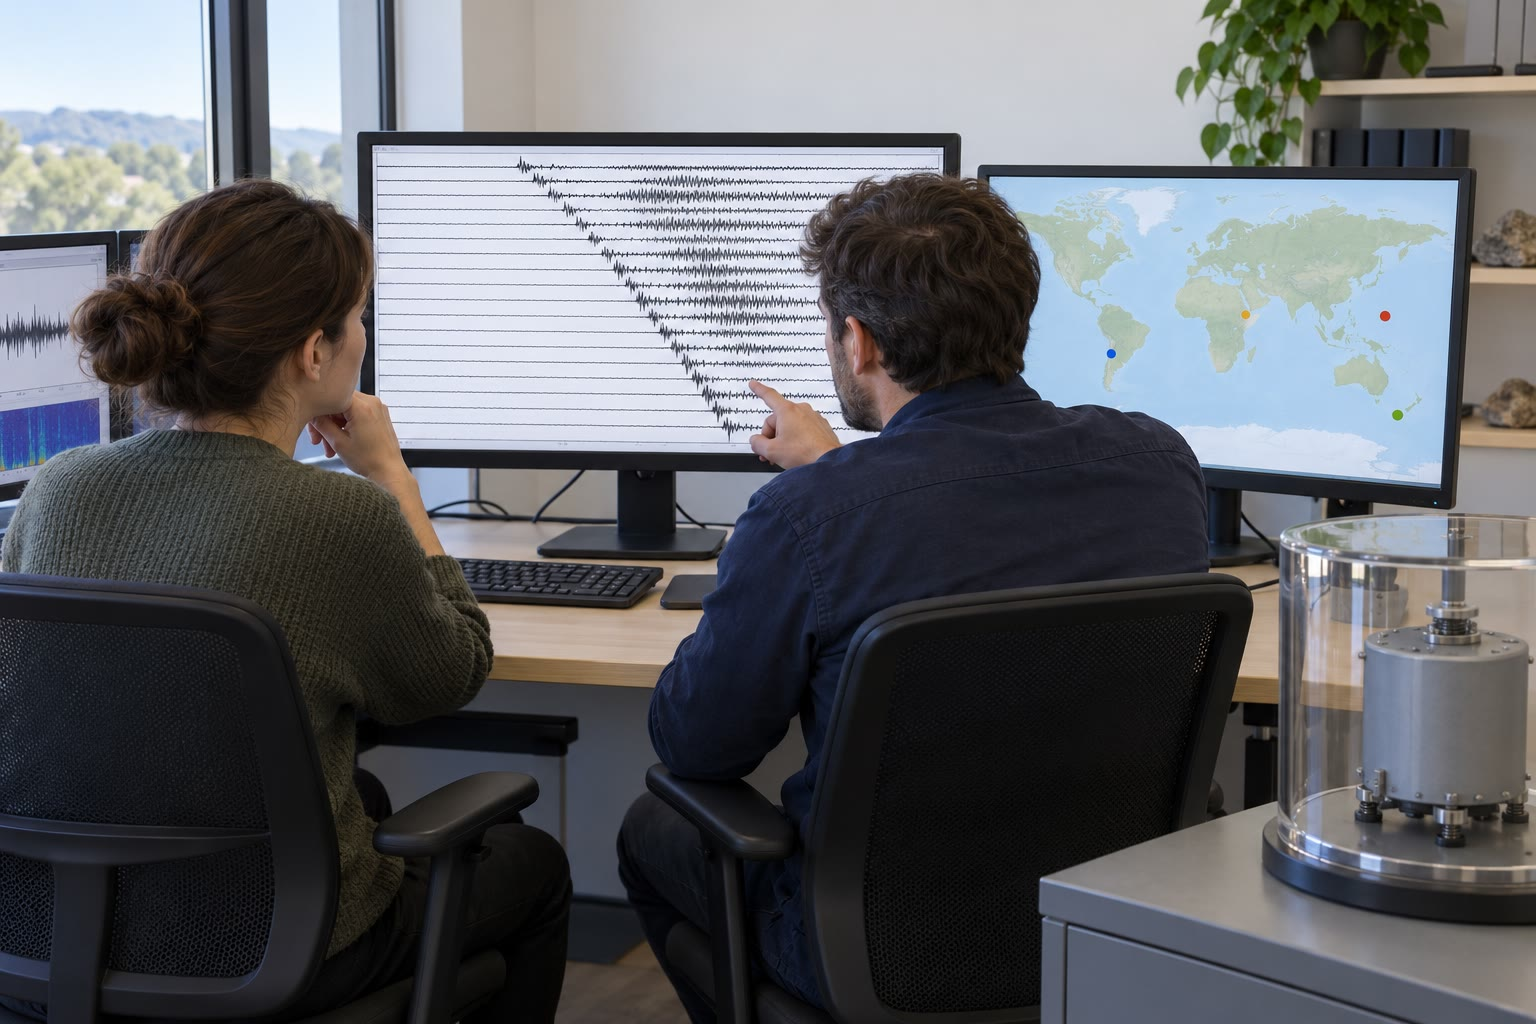
\includegraphics[width=\linewidth]{images/book3/ai/b1-seismic-analysis.jpg}

{\scriptsize علماء زلازل يقرؤون مقطعًا من التسجيلات، آثار زلزال واحد في محطات مرتّبة حسب المسافة (رسم بالذكاء الاصطناعي).}
\end{minipage}
\end{inthelab}
% ledger: yvo:beachball

\section{قياس التحميل: الجيوديزيا}\label{sec:b1:earthquake-source:geodesy}

بين الزلازل يكون الصدع المقفل غير مرئي لمقاييس الزلازل، لكن الأرض حوله تتحرّك. وتقيس محطات تحديد المواقع الدائمة بالأقمار الصناعية تلك الحركة، وطريقة تغيّر سرعاتها عبر الصدع تُخبر بمدى عمق قفله.

\begin{definition}[عمق القفل]\label{def:b1:earthquake-source:locking-depth}
\emph{عمق القفل}\index{عمق القفل} للصدع هو العمق الذي يبقى مقفلًا حتى حدّه بين الزلازل، والصدع تحته ينزلق انزلاقًا ثابتًا بالمعدّل طويل المدى؛ وهو عمق الجزء من الصدع الذي سينزلق في الزلزال التالي.
\end{definition}
% ledger: usgs:pp1515-thatcher

\begin{proposition}[السرعة البينية الزلزالية عبر صدع انزياحي]\label{prop:b1:earthquake-source:interseismic}
ليكن \omterm{def:b1:faults-folds-fabrics:fault-types}{صدع انزياحي} شاقولي، في نصف فضاء مرن، مقفلًا من السطح حتى العمق $D$، وينزلق بالمعدّل $V$ تحته. فسرعة السطح الموازية للصدع، على مسافة $x$ منه، هي
\[
  v(x) = \frac{V}{\pi}\arctan\frac{x}{D} .
\]
فإذا انزلق الصدع بعد ذلك بمقدار $s$ من السطح حتى العمق $D$ في زلزال، فإن السطح يتحرّك بالمقدار $u(x) = (s/\pi)\arctan(D/x)$ ل$x > 0$، وبالمقدار $-u(-x)$ ل$x < 0$.
\end{proposition}
\admitted

هذا النموذج، من عمل سافاج وبرفورد، هو أبسط صورة \omterm{def:b1:earthquake-source:seismic-cycle}{للارتداد المرن}، ومنحنى السور في الشكل الأول. وخصائصه تتبع من الصيغة.

\begin{proposition}[قراءة الملف البيني]\label{prop:b1:earthquake-source:profile}
في نموذج \cref{prop:b1:earthquake-source:interseismic}:
\begin{enumerate}[label=(\alph*)]
  \item بعيدًا عن الصدع تميل السرعة إلى $\pm V/2$، فتتحرّك الصفيحتان بسرعة $V$ بالنسبة لبعضهما؛
  \item نصف تغيّر السرعة عبر الصدع يحدث ضمن المسافة $D$ منه: $v(\pm D) = \pm V/4$؛
  \item معدّل \omterm{def:b1:stress-strain-rheology:strain}{انفعال القصّ} للسطح، $\mathrm dv/\mathrm dx$، يكون أكبر ما يكون على الصدع، حيث يساوي $V/(\pi D)$؛
  \item إذا انزلق الصدع، بعد التحميل لزمن $t$، بمقدار $s = Vt$ في زلزال، فإن الأرض تنتهي مُزاحةً بمقدار $\pm s/2$ في كل مكان على جانبيه: فالدورة لا تترك انحناءً دائمًا، بل الإزاحة $s$ على الصدع وحدها.
\end{enumerate}
\end{proposition}

\begin{proof}
(أ) $\arctan(x/D) \to \pm\pi/2$ عندما $x \to \pm\infty$. (ب) $\arctan 1 = \pi/4$، ف$v(D) = V/4$، و$v$ فردية. (ج) $\mathrm dv/\mathrm dx = (V/\pi D)/(1 +
x^2/D^2)$، أكبر ما يكون عند $x = 0$. (د) من أجل $x > 0$، حرّك التحميل الأرض بمقدار $t\,v(x) = (s/\pi)\arctan(x/D)$، والزلزال بمقدار $(s/\pi)\arctan(D/x)$؛ ولأن $\arctan y + \arctan(1/y) = \pi/2$ ل$y > 0$، فإن المجموع $s/2$. والأمر نفسه مع إشارات معكوسة ل$x < 0$.
\end{proof}

وتُعطي الخاصية (ب) \omterm{def:b1:earthquake-source:locking-depth}{عمق القفل} من ملفّ محطات: وهو المسافة عن الصدع التي يكون عندها تغيّر السرعة قد بلغ ربع $V$ من قيمتها على الصدع. فالقفل الضحل يركّز الانفعال قرب الصدع (الشكل أدناه)، والعميق ينشره على حزام عريض. وعلى طول نظام سان أندرياس، تتراوح أعماق القفل المستخرجة بالجيوديزيا من قرب الصفر، على المقاطع الزاحفة، حتى \qty{26}{km}، وتتّفق مع أعماق الزلازل: فالجزء المقفل هو \omterm{def:b1:stress-strain-rheology:strength-envelope}{الطبقة المولّدة للزلازل} في \cref{ch:b1:stress-strain-rheology}. وبالنسبة لمعدّل انزلاق قدره \qty{34}{mm.yr^{-1}} وعمق قفل قدره \qty{15}{km}، يكون معدّل \omterm{def:b1:stress-strain-rheology:strain}{انفعال القصّ} على الصدع $\num{0.034}/(\pi\times\num{15000}) = \num{7.2e-7}$ في السنة، وهو ما ينحني خطًّا عبر الصدع بأقلّ من مليمتر لكل كيلومتر في السنة، ومع ذلك يخزّن، عبر قرنين، الأمتار القليلة من انزلاق زلزال كبير.
% ledger: sk:mu-locking, usgs:pp1515-wallace, usgs:pp1515-thatcher

\begin{omfigure}
\begin{tikzpicture}[font=\small]
\begin{axis}[omrecord, width=11cm, height=5.6cm, xmin=-100, xmax=100, ymin=-19, ymax=19,
    xlabel={المسافة من الصدع $x$ (\unit{km})}, ylabel={السرعة $v$ (\unit{mm.yr^{-1}})},
    legend style={font=\scriptsize, at={(0.02,0.96)}, anchor=north west}, legend cell align=left]
  \addplot[omDef, line width=0.9pt, dashed] table[x=x, y=v5] {figdata/out/bachelor-1-interseismic-profiles.dat};
  \addplot[omThm, line width=1.1pt] table[x=x, y=v15] {figdata/out/bachelor-1-interseismic-profiles.dat};
  \addplot[omProp, line width=0.9pt, dotted] table[x=x, y=v25] {figdata/out/bachelor-1-interseismic-profiles.dat};
  \legend{$D = \qty{5}{km}$, $D = \qty{15}{km}$, $D = \qty{25}{km}$}
  \draw[black!50, dashed] (axis cs:-100,17) -- (axis cs:100,17);
  \draw[black!50, dashed] (axis cs:-100,-17) -- (axis cs:100,-17);
  \node[anchor=north west, font=\scriptsize] at (axis cs:-30,17) {$+V/2$};
  \node[anchor=south west, font=\scriptsize] at (axis cs:30,-17) {$-V/2$};
  \draw[black!60] (axis cs:0,-19) -- (axis cs:0,19);
  \node[anchor=east, font=\scriptsize] at (axis cs:-1,5) {الصدع};
\end{axis}
\end{tikzpicture}
\par\smallskip{\small سرعة الأرض الموازية \omterm{def:b1:faults-folds-fabrics:fault-types}{لصدع انزياحي} مقفل، بالنسبة لأثر الصدع، من أجل معدّل انزلاق $V = \qty{34}{mm.yr^{-1}}$، وهو معدّل صدع سان أندرياس عند جدول وولاس، وثلاثة أعماق قفل (\cref{prop:b1:earthquake-source:interseismic}). فكلما كان القفل أضحل، كان الحزام الذي تتغيّر فيه السرعة أضيق.}
\label{fig:b1:earthquake-source:interseismic}
\end{omfigure}
% ledger: usgs:pp1515-wallace

تقيس الأقمار الصناعية للرادار الأرض في كل مكان: تُقارَن صورتان رادارّيتان للمنطقة نفسها، أُخذتا من المدار نفسه في زمنين مختلفين، موجةً بموجة، ويرسم فرق الطَّور تغيّر المسافة بين الأرض والقمر الصناعي، نقطةً بنقطة، على مسافات مئة متر، دون شبكة محطات تُنشأ مسبقًا. وأول خريطة من هذا النوع، لزلزال كاليفورني كبير عام 1992، أظهرت إزاحته المشاركة للزلزال في صورة واحدة، واتفقت مع الانزلاق المقاس في الميدان وبالمسح؛ والتقنية، التداخل الرادري، من اختصاص المجلد الثالث.
% ledger: massonnet:1993

\section{كم مرة: قانون غوتنبرغ--ريختر}\label{sec:b1:earthquake-source:gr}

الزلازل الصغيرة أكثر بكثير من الكبيرة، وبطريقة منتظمة بشكل لافت.

\begin{proposition}[قانون غوتنبرغ--ريختر]\label{prop:b1:earthquake-source:gutenberg-richter}
في منطقة وفترة زمنية\index{قانون غوتنبرغ--ريختر}، يتبع العدد $N$ من الزلازل التي قدرها على الأقل $M$ الصيغةَ الآتية:
\[
  \log_{10} N = a - bM ,
\]
لكل $M$ فوق \omterm{def:b1:earthquake-source:b-value}{حدّ الاكتمال} للكتالوج، مع ثابتين $a$ و$b$ يتعلّقان بالمنطقة؛ و$b$ قريب من 1 في معظم المناطق النشطة.
\end{proposition}
\admitted
% ledger: fd:1993, gr:1944

القانون نتيجة ملاحظة، نشرها بينو غوتنبرغ وتشارلز ريختر لكاليفورنيا عام 1944، ووُجدت منذ ذلك الحين في كل مكان؛ ولم تستنتجه بعد أيّ نظرية، ولا قيمة $b$.
% ledger: gr:1944

\begin{definition}[قيمة b، وحدّ الاكتمال]\label{def:b1:earthquake-source:b-value}
الثابت $b$ \omterm{prop:b1:earthquake-source:gutenberg-richter}{لقانون غوتنبرغ--ريختر} لمنطقة هو \emph{قيمة b}\index{قيمة b}. و\emph{حدّ الاكتمال}\index{حدّ الاكتمال} لكتالوج هو أصغر قدر يسجّل فوقه كل زلزال في المنطقة والفترة.
\end{definition}

\omterm{def:b1:earthquake-source:b-value}{قيمة b} تساوي 1 تعني عشر مرات أقلّ من الزلازل مع كل وحدة من القدر. وتحت \omterm{def:b1:earthquake-source:b-value}{حدّ الاكتمال}، تقع الأعداد تحت الخطّ، لأن الزلازل الصغيرة تسجّلها محطات قليلة جدًّا لتحديد موضعها: فيبدو القانون منحنيًا، ويجب أن تُقاس $b$ فوقه. وبالنسبة للأرض كلها، مقسّمةً إلى زلازل ضحلة ومتوسطة وعميقة، تقع القيم المقاسة بين 0.72 و\num{1.34}، لكنها تختلف ب\qty{30}{\percent} أو أكثر من كتالوج إلى آخر، أو من مدى قدر إلى آخر، أو من طريقة إلى أخرى: فقيمة بعيدة عن 1 هي أول سبب للتحقّق من الكتالوج.
% ledger: fd:1993

\begin{omfigure}
\begin{tikzpicture}[font=\small]
\begin{axis}[omrecord, width=6.4cm, height=5.8cm, ymode=log, xmin=5.8, xmax=9.3, ymin=0.01, ymax=300,
    xlabel={القدر $M$}, ylabel={عدد الزلازل التي قدرها $\ge M$ في السنة},
    log basis y=10, title={(أ) التواتر والقدر}, title style={font=\small}]
  \addplot[omProp, line width=0.9pt, domain=5.8:9.3] table[x=M, y=rate] {figdata/out/bachelor-1-gutenberg_richter-fit.dat};
  \addplot[only marks, mark=*, mark size=1.3pt, omDef] table[x=M, y=rate] {figdata/out/bachelor-1-gutenberg_richter-counts.dat};
  \draw[black!50, dashed] (axis cs:7.5,0.01) -- (axis cs:7.5,300);
  \node[anchor=south west, font=\scriptsize, omProp] at (axis cs:8.45,0.5) {$b = 1.01$};
  \node[anchor=north west, font=\scriptsize, align=left] at (axis cs:7.55,200) {مُطابَق على\\ $6.0 \le M \le 7.5$};
\end{axis}
\begin{axis}[omrecord, at={(7.6cm,0)}, width=6.4cm, height=5.8cm, xmin=5.8, xmax=9.3, ymin=0, ymax=1.05,
    xlabel={القدر $M$}, ylabel={نسبة العزم من الزلازل التي قدرها $\ge M$},
    title={(ب) أين يذهب العزم}, title style={font=\small}]
  \addplot[const plot, omDef, line width=0.9pt] table[x=M, y=share] {figdata/out/bachelor-1-gutenberg_richter-moment.dat};
\end{axis}
\end{tikzpicture}
\par\smallskip{\small \num{7031} زلزالًا قدره 6 أو أكثر في العالم، 1976--2025 (كتالوج هيئة المسح الجيولوجي الأمريكية). (أ) العدد السنوي للزلازل التي قدرها $M$ على الأقل؛ والخطّ هو المطابقة بالمربعات الصغرى ل$\log_{10} N$ على $M$ من 6.0 إلى 7.5، حيث يتجاوز كل عدد 200: $\log_{10} N = 8.20 - 1.01\,M$ في السنة. وفوق القدر 8 تقع الأحداث القليلة تحت الخطّ. (ب) نسبة مجموع \omterm{def:b1:earthquake-source:moment}{العزم الزلزالي} المُطلَق من الزلازل التي قدرها $M$ على الأقل، إذ يُحسب كل عزم ب$10^{1.5M + 9.1}$\,\unit{N.m}: الأربعون زلزالًا التي قدرها 8 أو أكثر أطلقت \qty{63}{\percent} منه.}
\label{fig:b1:earthquake-source:gutenberg-richter}
\end{omfigure}
% ledger: data:usgs-comcat (fit and shares computed in figdata/bachelor-1/gutenberg_richter.py)

بالنسبة لكتالوج العالم في الشكل، يتنبّأ القانون ب$a = 8.20$ و$b = 1.01$ ب\num{14} زلزالًا قدره 7 أو أكثر في السنة، كما يُلاحَظ، وب\num{1.35} قدره 8 أو أكثر، بينما سُجّل 40 في خمسين سنة، أي 0.8 في السنة. وهل الزلازل الكبرى أقلّ فعلًا من الخطّ، كما يوحي الحجم المحدود للصدوع، أم أنها نادرة إلى حدّ أن تغيب عن خمسين سنة، فهذا لا يُحسم بعدد قليل من الأحداث هكذا. وقرابة واحد من كل تسعة قدرات في هذا الكتالوج هو قدر موجات سطحية أو جسمية، وهي تتشبّع؛ وأكبر الأحداث كلها لها قدرات عزم.
% ledger: data:usgs-comcat

الزلازل الصغيرة الكثيرة لا تؤدّي إلا القليل من العمل. فعددها ينمو عشر مرات مع كل وحدة من القدر أقلّ، لكن عزومها تتقلّص 31.6 مرة.

\begin{proposition}[أكبر الزلازل تُطلق معظم العزم]\label{prop:b1:earthquake-source:largest}
لتتبع الزلازلُ \omterm{prop:b1:earthquake-source:gutenberg-richter}{قانون غوتنبرغ--ريختر} مع $b < 1.5$، حتى قدر أكبر $M_{\max}$، ولتُجمَّع في فئات عرض كل منها وحدة واحدة من القدر، وتنتهي الفئة العليا عند $M_{\max}$. فإن زلازل الفئة العليا تطلق أكثر من الكسر $1 - 10^{-(1.5 - b)}$ من مجموع العزم، مهما كان أصغر قدر محسوب صغيرًا: أكثر من \qty{68}{\percent} عندما $b = 1$.
\end{proposition}

\begin{proof}
لتُرقَّم الفئات $k = 0, 1, \dots, K$ من الأصغر، وتمتدّ الفئة $k$ من $M_k$ إلى $M_k + 1$، مع $M_{k+1} = M_k + 1$. بحسب القانون، عدد الزلازل في الفئة $k$ هو $10^{a - bM_k} - 10^{a - b(M_k+1)} =
10^{a - bM_k}(1 - 10^{-b})$؛
وبحسب \cref{prop:b1:earthquake-source:moment-steps} يقع عزم كلٍّ منها بين $10^{1.5M_k + 9.1}$ و$10^{1.5}$ مضروبًا فيه، ولأن كل فئة هي الفئة السابقة مُزاحةً بوحدة واحدة، فإن عزم الفئة $k$ هو $C q^k$ لثابت $C$، والنسبة $q = 10^{-b}\times10^{1.5} = 10^{1.5 - b} > 1$. والمجموع هو المتتالية الهندسية
\[
  S = C(1 + q + \dots + q^K) = C\,\frac{q^{K+1} - 1}{q - 1} ,
\]
ونسبة الفئة العليا هي
\[
  \frac{C q^K}{S} = \frac{q^K (q - 1)}{q^{K+1} - 1}
  > \frac{q^K (q - 1)}{q^{K+1}} = 1 - \frac1q = 1 - 10^{-(1.5 - b)} .
\]
من أجل $b = 1$، يكون $1 - 10^{-0.5} = 0.684$.
\end{proof}

في كتالوج العالم تكون النسبة من هذا الترتيب: فالوحدة القدرية العليا، من 8.1 إلى 9.1، أطلقت أكثر من نصف عزم الخمسين سنة، وأكبر زلزالين، سومطرة--أندامان عام 2004 وتوهوكو عام 2011، بقدر 9.1 لكلٍّ منهما، أطلقا وحدهما \qty{29}{\percent} منه. والعزم الذي يجب أن يُطلقه حدّ صفيحة تحدّده سرعة انزلاقه؛ والقضية تقول إنه يُطلَق كله تقريبًا في أكبر زلازله، وأن الزلازل الصغيرة الكثيرة، مهما كانت متكررة، لا تُخفّف عن الصدع الزلزال الكبير التالي.
% ledger: data:usgs-comcat, usgs:sumatra-mt, usgs:tohoku-mt

\section{التمارين}

\begin{exercise}[$\star$]\label{exo:b1:earthquake-source:1}
(أ) احسب \omterm{def:b1:earthquake-source:mw}{قدر العزم} لزلزال \omterm{def:b1:earthquake-source:moment}{عزمه الزلزالي} \qty{4e17}{N.m}. (ب) كان لزلزال توهوكو $M_0 = \qty{5.59e22}{N.m}$: تحقّق من قدره. (ج) ما \omterm{def:b1:earthquake-source:moment}{العزم الزلزالي} لزلزال قدره 7.0؟
% ledger: usgs:tohoku-mt
\end{exercise}

\begin{exercise}[$\star$]\label{exo:b1:earthquake-source:2}
\omterm{def:b1:faults-folds-fabrics:fault-types}{صدع انزياحي} يُحمَّل بمعدّل \qty{25}{mm.yr^{-1}}، وينزلق كل زلزال منه بنحو \qty{3}{m}. (أ) ما فترة تكراره إن كان الصدع مقفلًا تمامًا بينها؟ (ب) وإن أُخذ نصف معدّل الانزلاق بزحف ثابت؟
\end{exercise}

\begin{exercise}[$\star$]\label{exo:b1:earthquake-source:3}
كم مرة أكبر \omterm{def:b1:earthquake-source:moment}{العزم الزلزالي} لزلزال قدره 7.4 من زلزال قدره 6.2؟ وكم زلزالًا قدره 6.2 يُطلق العزم نفسه؟
\end{exercise}

\begin{exercise}[$\star$]\label{exo:b1:earthquake-source:4}
في منطقة فيها $b = 1$، يُسجَّل ألف زلزال قدره 3 أو أكثر كل سنة. كم زلزالًا قدره 5 أو أكثر، وكم قدره 6 أو أكثر، يُتوقّع كل سنة؟ وما متوسط الزمن بين الزلازل التي قدرها 7 أو أكثر؟
\end{exercise}

\begin{exercise}[$\star\star$]\label{exo:b1:earthquake-source:5}
كسر زلزال 1906 صدع سان أندرياس على نحو \qty{430}{km}. (أ) بافتراض أن الانكسار بلغ عمق \qty{15}{km} بانزلاق متوسطه \qty{4}{m}، و$\mu = \qty{30}{GPa}$، احسب \omterm{def:b1:earthquake-source:moment}{عزمه الزلزالي} وقدره العزمي. (ب) كم يتغيّر القدر إن كان الانكسار عميقًا \qty{10}{km} فقط؟ (ج) أيّ التقديرين أقرب إلى 7.9؟
% ledger: pp1515:1906, usgs:hist-mw
\end{exercise}

\begin{exercise}[$\star\star$]\label{exo:b1:earthquake-source:6}
بلغ انكسار زلزال توهوكو نحو \qty{400}{km} طولًا و\qty{150}{km} عرضًا، وعزمه \qty{5.59e22}{N.m}. (أ) احسب متوسط انزلاقه ب$\mu = \qty{30}{GPa}$. (ب) تغوص الصفيحة الباسيفيكية تحت اليابان بنحو \qty{83}{mm.yr^{-1}}: كم يستغرق تراكم هذا الانزلاق إن كانت الواجهة مقفلة تمامًا؟ (ج) وإن كان الكسر المقفل 0.8، أو 0.5؟
% ledger: usgs:tohoku-mt, usgs:tohoku-summary
\end{exercise}

\begin{exercise}[$\star\star$]\label{exo:b1:earthquake-source:7}
أحد المستويين العقديين لزلزال سومطرة--أندامان عام 2004 امتداده $329$، وانحداره \ang{8}، وزاوية انزلاقه \ang{110}. (أ) اكتب $\mathbf n$ و$\mathbf d$ بمركّبات شرقية وشمالية وعلوية. (ب) أوجد \omterm{def:b1:geological-maps:attitude}{الامتداد} \omterm{def:b1:geological-maps:attitude}{والانحدار} \omterm{def:b1:faults-folds-fabrics:fault-elements}{وزاوية الانزلاق} للمستوى المساعد. (ج) أوجد اتجاهي محوري P وT وغوصيهما. (د) أيّ المستويين هو الصدع، وأيّ نوع من الصدوع هو؟
% ledger: usgs:sumatra-mt
\end{exercise}

\begin{exercise}[$\star\star$]\label{exo:b1:earthquake-source:8}
صدع شاقولي يمتدّ $045$ ينزلق انزلاقًا \omterm{def:b1:faults-folds-fabrics:fault-types}{أيمن}. (أ) للموجات التي تغادر البؤرة أفقيًّا نحو محطات تقع شمالًا وشرقًا وجنوبًا وغربًا، أيّها تصل كدفعات وأيّها كسحوب؟ (ب) أعطِ اتجاهي محوري P وT. (ج) بيّن أن انزلاقًا \omterm{def:b1:faults-folds-fabrics:fault-types}{أيسر} على مستوى شاقولي يمتدّ $135$ يعطي الحركات الأولى نفسها.
\end{exercise}

\begin{exercise}[$\star\star$]\label{exo:b1:earthquake-source:9}
عبر \omterm{def:b1:faults-folds-fabrics:fault-types}{صدع انزياحي} مقفل، تتحرّك المحطات البعيدة على الجانبين بالنسبة لبعضها بمعدّل \qty{40}{mm.yr^{-1}}. وتتحرّك محطة على بُعد \qty{10}{km} من الصدع بمعدّل \qty{10}{mm.yr^{-1}} بالنسبة لأثر الصدع. (أ) أوجد \omterm{def:b1:earthquake-source:locking-depth}{عمق القفل}. (ب) تنبّأ بسرعة محطة على بُعد \qty{30}{km} من الصدع. (ج) احسب معدّل \omterm{def:b1:stress-strain-rheology:strain}{انفعال القصّ} على الصدع.
\end{exercise}

\begin{exercise}[$\star\star\star$]\label{exo:b1:earthquake-source:10}
(أ) بيّن أنه لو كان $b$ أكبر من 1.5، لهيمن على العزم الكلّي لزلازل منطقة أصغرُ زلازلها. (ب) ما أدنى نسبة من العزم تطلقها الوحدة القدرية العليا، من أجل $b = 0.8$؟ (ج) بالقيمتين $a = 8.20$ و$b = 1.01$ في السنة لكتالوج العالم، كم زلزالًا قدره 9 أو أكثر يتنبّأ به القانون في خمسين سنة؟ ويحوي كتالوج 1976--2025 اثنين؛ علِّق.
% ledger: data:usgs-comcat
\end{exercise}

\begin{exercise}[$\star\star\star$]\label{exo:b1:earthquake-source:11}
يُبنى سور مستقيم عبر صدع \omterm{def:b1:faults-folds-fabrics:fault-types}{أيمن} مقفل ب$V =
\qty{34}{mm.yr^{-1}}$ و$D = \qty{15}{km}$. (أ) بعد 150 سنة، بكم تحرّكت الأعمدة على بُعد \qty{1}{km}، و\qty{15}{km}، و\qty{50}{km} شرق الصدع، على طوله، بالنسبة للعمود الواقع على الصدع؟ (ب) ينزلق الصدع بعد ذلك بكامل العجز في زلزال. ما الانزلاق، وبكم يتحرّك كلّ عمود من الثلاثة في الزلزال؟ (ج) تحقّق من الجزء (د) من \cref{prop:b1:earthquake-source:profile} على الأعمدة الثلاثة.
% ledger: usgs:pp1515-wallace
\end{exercise}

\begin{exercise}[$\star\star\star$]\label{exo:b1:earthquake-source:12}
لزلزال \omterm{def:b1:earthquake-source:focal-mechanism}{محور P} أفقي يتّجه $000$، \omterm{def:b1:earthquake-source:focal-mechanism}{ومحور T} أفقي يتّجه $090$. (أ) بيّن أن مستويَيه العقديين شاقوليان، وامتدادهما $045$ و$135$، باستعمال $\mathbf n$، و$\mathbf d = (\mathbf T \pm \mathbf P)/\sqrt2$. (ب) أعطِ اتجاه الانزلاق على كل مستوى. (ج) لو تكوّن الصدع جديدًا في صخر فيه $\phi = \ang{30}$، تحت $\sigma_1$ على طول \omterm{def:b1:earthquake-source:focal-mechanism}{محور P}، فعند أيّ امتدادات كان سيقع، ولماذا \omterm{def:b1:earthquake-source:focal-mechanism}{محور P} تقريب فقط ل$\sigma_1$؟ (د) صدع مرسوم قريب يمتدّ $040$. أيّ المستويين العقديين هو الصدع على الأرجح، وما اتجاه انزلاقه؟
\end{exercise}

\section{مسألة: الزلزال الكبير التالي على صدع مقفل}

\begin{problem}[{مسألة نهاية الأسبوع: قطعة مقفلة من حدّ صفيحة انزياحي، من تحميلها وزلازلها الماضية إلى قدر التالي}]
\label{pb:b1:earthquake-source:1}
% values: calc/ch18.py; an invented fault (the numbers are of a realistic order)
\omterm{def:b1:faults-folds-fabrics:fault-types}{صدع انزياحي} مستقيم شاقولي يشكّل حدًّا بين صفيحتين. وإحدى قطعه، طولها \qty{250}{km}، مقفلة؛ وزلازلها تبدأ على عمق لا يزيد عن \qty{15}{km}. وقد حفرت خنادق عبره، فأرّخت آخر أربعة زلازل كبيرة فيها بنحو 1050 و\num{1290} و\num{1480} و\num{1712}، بإزاحات قدرها \num{7.0} و\num{6.0} و\num{5.5} و\qty{7.5}{m}. وتتحرّك المحطات الدائمة البعيدة عن الصدع على الجانبين بالنسبة لبعضها بمعدّل \qty{30}{mm.yr^{-1}}. خذ $\mu =
\qty{30}{GPa}$، والسنة 2025 هي الحاضر، وأعطِ الأقدار حتى 0.01.

\medskip
\noindent\textbf{الجزء الأول --- التحميل.}
\begin{enumerate}
  \item احسب الفواصل بين الزلازل الأربعة ومتوسطها.
  \item احسب متوسط الإزاحة، \omterm{def:b1:earthquake-source:seismic-cycle}{وفترة التكرار} التي تقتضيها ب\cref{prop:b1:earthquake-source:recurrence} لصدع مقفل بالكامل.
  \item احسب معدّل الانزلاق الذي يقتضيه الخندق وحده، من إزاحات الزلازل الثلاثة الأخيرة والزمن بين الأول والأخير. قارن بالمعدّل الجيوديزي.
  \item منذ متى كان آخر زلزال، وما عجز الانزلاق الذي تراكم منذ ذلك الحين، إن كانت القطعة مقفلة تمامًا؟
  \item قارن هذا العجز بالإزاحات في الخندق. هل الزلزال التالي متأخّر؟
  \item لماذا لا يستطيع الخندق أن يعطي تاريخ التالي؟
\end{enumerate}

\medskip
\noindent\textbf{الجزء الثاني --- حجم الزلزال التالي.}
\begin{enumerate}[resume]
  \item ما مساحة الجزء المقفل من القطعة؟
  \item احسب \omterm{def:b1:earthquake-source:moment}{العزم الزلزالي} لزلزال يطلق العجز كله.
  \item احسب \omterm{def:b1:earthquake-source:mw}{قدر العزم} لزلزال 1712، بافتراض أنه كسر المساحة نفسها، وأن إزاحته في الخندق هي الانزلاق المتوسّط.
  \item بأيّ عامل يتجاوز عزم الزلزال التالي عزم زلزال 1712، وكم وحدة قدرية هذا؟
  \item لو انكسر نصف القطعة فقط، بالانزلاق نفسه، فما يكون القدر؟
  \item أعطِ \omterm{def:b1:earthquake-source:moment}{العزم الزلزالي} الذي تتراكمه القطعة كل سنة.
\end{enumerate}

\medskip
\noindent\textbf{الجزء الثالث --- التواتر والطاقة.}
\begin{enumerate}[resume]
  \item يتبع الكتالوج الإقليمي $\log_{10} N = 4.3 - M$ في السنة، من جميع صدوع المنطقة. ما \omterm{def:b1:earthquake-source:b-value}{قيمة b}، وكم زلزالًا قدره 5 أو أكثر، وقدره 6 أو أكثر، يعطي كل سنة؟
  \item ما متوسط الزمن بين الزلازل التي قدرها 7 أو أكثر، وقدرها 8 أو أكثر، الذي يعطيه؟
  \item قارن تكرار زلزال كبير من الكتالوج بتكراره من الخندق. ماذا يقول الفرق عن استعمال قانون الزلازل الصغيرة للتنبّؤ بالكبيرة؟
  \item تُطلق الزلازل التي قدرها بين 5 و\num{8} من قانون المنطقة الإقليمي، مجتمعةً، نحو \qty{5.5e17}{N.m} في السنة. ما الكسر الذي تمثّله من عزم القطعة؟
  \item كم مرة أكثر من الطاقة التي يشعّها زلزال قدره 6 سيشعّ الزلزال الكبير التالي؟
  \item باستعمال \cref{prop:b1:earthquake-source:largest}، اشرح لماذا لا تُخفّف الزلازل المعتدلة في القطعة عنها.
\end{enumerate}

\medskip
\noindent\textbf{الجزء الرابع --- \omterm{def:b1:earthquake-source:locking-depth}{عمق القفل} من المحطات.}
\begin{enumerate}[resume]
  \item يعطي ملفّ محطات عبر القطعة، بالنسبة لأثر الصدع، السرعات $-11.6$، $-7.5$، $-3.1$، $3.1$، $7.5$ و\qty{11.6}{mm.yr^{-1}} عند $x = -40$، $-15$، $-5$، $5$، $15$ و\qty{40}{km}. تحقّق أن الملفّ ضدّ متماثل، واعطِ السرعات المتوقّعة بعيدًا عن الصدع.
  \item من المحطة عند \qty{15}{km}، احسب \omterm{def:b1:earthquake-source:locking-depth}{عمق القفل}.
  \item احسبه مرة أخرى من المحطتين عند \qty{5}{km} و\qty{40}{km}، واشرح الفروق الصغيرة.
  \item قارن \omterm{def:b1:earthquake-source:locking-depth}{عمق القفل} بعمق الزلازل، وقُل لماذا ينبغي أن يتّفقا.
  \item احسب معدّل \omterm{def:b1:stress-strain-rheology:strain}{انفعال القصّ} على الصدع.
  \item لأقرب 0.01، ما \omterm{def:b1:earthquake-source:mw}{قدر العزم} للزلزال الذي يطلق عجز الانزلاق كله في القطعة؟
\end{enumerate}
\end{problem}
